
%(BEGIN_QUESTION)
% Copyright 2011, Tony R. Kuphaldt, released under the Creative Commons Attribution License (v 1.0)
% This means you may do almost anything with this work of mine, so long as you give me proper credit

HART instruments have the capability of operating as purely digital devices, with no analog current signal output.  When multiple HART devices are operated like this, paralleled on a common network cable, it is called {\it multidrop mode}:

$$\includegraphics[width=15.5cm]{i02229x01.eps}$$

Answer the following questions about ``multidropped'' HART instruments:

\begin{itemize}
\item{} Explain why multidrop HART mode precludes the use of 4-20 mA as a signaling standard.  In other words, explain why the option of ``multidropping'' HART instruments is an {\it all-or-nothing} choice, rendering the loop current signal meaningless with regard to process measurements.
\vskip 10pt
\item{} Explain why each HART instrument in multidrop mode requires a unique ``address'' number assigned to it, and identify how many (maximum) different addresses may exist in a HART multidrop network.
\vskip 10pt
\item{} Explain why ``burst mode'' cannot be used with multidrop HART instruments, and then identify applications where burst mode {\it would} be useful.
\vskip 10pt
\item{} Finally, identify at least three different places in this network where a HART modem or handheld communicator could be connected to establish communication with the devices. 
\end{itemize}

\vskip 20pt \vbox{\hrule \hbox{\strut \vrule{} {\bf Suggestions for Socratic discussion} \vrule} \hrule}

\begin{itemize}
\item{} How much total current would you expect to measure in a multidrop HART network?
\item{} What is the maximum number of HART devices that may be multi-dropped?
\end{itemize}


\underbar{file i02229}
%(END_QUESTION)





%(BEGIN_ANSWER)

The reason why we must abandon 4-20 mA signaling in a multidrop HART network should be obvious if you understand the characteristics of parallel DC circuits: the total current is the {\it sum} of all branch currents.

\vskip 10pt

Unique HART addresses are necessary to ensure the ability to communicate to and from specific transmitters, one at a time.

\vskip 10pt

In burst mode, the field instrument does not wait to be polled by a master device; instead, it continually broadcasts data to the HART network.

\vskip 10pt

You may connect a HART modem or communicator in the following locations in a multidrop network:

\begin{itemize}
\item{} In parallel with the two wires, anywhere along the cable length
\item{} In parallel with the connection terminals of instrument \#1
\item{} In parallel with the connection terminals of instrument \#2
\item{} In parallel with the connection terminals of instrument \#3
\item{} In parallel with the resistor
\end{itemize}

\vskip 10pt

Unique addressing is required because this ``bus'' network is {\it broadcast} by nature.

%(END_ANSWER)





%(BEGIN_NOTES)

In ``multidrop'' mode, each transmitter draws a constant 4 mA of current: just enough to power the internal circuitry.  Total current is therefore equal to the number of devices multiplied by 4 mA.

\vskip 10pt

The maximum number of HART field devices in a multidrop network is 15: 1 through 15, with the address 0 reserved for the Master device (modem or handheld communicator).

\vskip 20pt \vbox{\hrule \hbox{\strut \vrule{} {\bf Virtual Troubleshooting} \vrule} \hrule}

This question is a good candidate for a ``Virtual Troubleshooting'' exercise.  Presenting the diagram to students, you first imagine in your own mind a particular fault in the system.  Then, you present one or more symptoms of that fault (something noticeable by an operator or other user of the system).  Students then propose various diagnostic tests to perform on this system to identify the nature and location of the fault, as though they were technicians trying to troubleshoot the problem.  Your job is to tell them what the result(s) would be for each of the proposed diagnostic tests, documenting those results where all the students can see.

During and after the exercise, it is good to ask students follow-up questions such as:

\begin{itemize}
\item{} What does the result of the last diagnostic test tell you about the fault?
\item{} Suppose the results of the last diagnostic test were different.  What then would that result tell you about the fault?
\item{} Is the last diagnostic test the best one we could do?
\item{} What would be the ideal order of tests, to diagnose the problem in as few steps as possible?
\end{itemize}

%INDEX% Fieldbus, HART: multidrop mode

%(END_NOTES)


